% !TeX TXS-program:compile = txs:///pdflatex/[--shell-escape]

\documentclass[9pt]{beamer}
\usetheme{Madrid}
\usecolortheme{beaver}
\usepackage{amsmath,amssymb,amsthm,asymptote,graphicx}
\usepackage{graphics}
% \usepackage{bisvslides}
\usepackage{arcs}
\usepackage{tikz}
\graphicspath{{./images}}

\newcounter{problem}[section]

\newenvironment{probslide}[3][]{%
    \refstepcounter{problem}\begin{frame}[t]%
	{Problem \thesection.\theproblem 
        \def\temp{#2}\ifx\temp\empty
            %
        \else
            \ - \temp%
        \fi}
    {#3}}%
	{\end{frame}}

% \newenvironment{Example}[2][Example]
%     {This is an #1. You gave #2 as an argument. The rest will be bold: \bfseries}
%     {}
% \textbf{Problem~\theproblem. #1
% \newenvironment{bsmi}{\begin{CJK}{UTF8}{bsmi}}{\end{CJK}}

\title{Geometry}
\subtitle{Mathcounts 22 - Session 3}
\author{Irene W., Pranav B., Brianna Z., Derrick L.}
\institute{BISV Mathcounts Club 22}
\date{December 13, 2022}

%\maketitle
%~~~~~~~~~~~~~~~~~~~~~~~~~~~~~~~~~~~~~~~~~~~~~~~~~~~~~~~~~~~~~~~~~~~~~~~~~~~~~~
% Informations
%\title{TEMPLATE}

%\titlegraphic{assets/gkg.png} %change this to your preferred logo or image(the image is located on the top right corner).
%~~~~~~~~~~~~~~~~~~~~~~~~~~~~~~~~~~~~~~~~~~~~~~~~~~~~~~~~~~~~~~~~~~~~~~~~~~~~~~

\begin{document}

% Generate title page
\begin{frame}
    \titlepage        
\end{frame}
% \setbeamertemplate{footline}[miniframes Madrid]

\setcounter{section}{7}

\section{Beginner Practice Problems}
\refstepcounter{problem}
\begin{frame}[t, fragile]{Problem \thesection.\theproblem}
    \begin{block}{} [Mathcounts 2008 School, Target \#2]
Square $A$ has a perimeter of $24$ cm. Square $B$ has an area equal to one-fourth of the area of Square $A$. What is the perimeter of square $B$
        

    \end{block}
\end{frame}

\refstepcounter{problem}
\begin{frame}[t, fragile]{Problem \thesection.\theproblem}
    \begin{block}{}
    Given a 30-60-90 triangle with hypotenuse length 20, what is the area of the triangle? Give your answer in the simplest radical form
	
    \end{block}
\end{frame}
\refstepcounter{problem}
\begin{frame}[t, fragile]{Problem \thesection.\theproblem}
    \begin{block}{}
    Mary is standing at the edge of a 10 foot wide river and sees her friend Cherisa across the river and 10 feet to the right from where Mary is standing. What is the shortest distance between Mary and Cherisa? Round your answer to the nearest tenth
    
    \end{block}
\end{frame}
\refstepcounter{problem}
\begin{frame}[t, fragile]{Problem \thesection.\theproblem}
    \begin{block}{}
    10 concentric circles, with radii 1,2,3,...,10 are shaded alternating black and white colors, with the circle of radius 1 being shaded black. For example, the area of the circle with radius 2 outside the circle with radius 1 and inside the circle with radius 2 would be colored white, and so one. There is no overlap between the coloring of the circles. What is the combine area of the white circles? Leave your answer in terms of $ \pi $.
    
    \end{block}
\end{frame}
\refstepcounter{problem}
\begin{frame}[t, fragile]{Problem \thesection.\theproblem}
    \begin{block}{}
    A right pyramid has height 7.5, and its base triangle is a right triangle with base length 3.4 and height 6.1. Find the volume of the tetrahedron. Round your answer to the nearest whole number.
    
    \end{block}
\end{frame}
\refstepcounter{problem}
\begin{frame}[t, fragile]{Problem \thesection.\theproblem}
    \begin{block}{}
    (Mathcounts) What is the minimum number of equilateral triangles, of side length 1 unit, needed to cover an equilateral triangle of side length 10 units?
    
    \end{block}
\end{frame}



\refstepcounter{problem}
\begin{frame}[t, fragile]{Problem \thesection.\theproblem}
    \begin{block}{}
    (Mathcounts) Quadrilateral $ABCD$ is inscribed in circle $O$ as shown. Arc $AB = 100$ degrees, and arc $BC = 50$ degrees. What is the measure of angle $ADC$?
    \end{block}
    \begin{center}
        \includegraphics[scale=0.4]{915669443e24631474bf80a6c6e4084b6a6668ec.png}
    \end{center}
    

\end{frame}

\refstepcounter{problem}
\begin{frame}[t, fragile]{Problem \thesection.\theproblem}
    \begin{block}{}
    (Mathcounts) In the figure below, isosceles $\triangle ABC$ with base $\overline{AB}$ has altitude $CH = 24$ cm. $DE = GF$, $HF = 12$ cm, and $FB = 6$ cm. What is the number of square centimeters in the area of pentagon $CDEFG$?
    
    \end{block}
    \begin{center}
        \includegraphics[scale=0.4]{dcfaf4dab16fff71a2813f8c7f8bc6417390e865.png}
    \end{center}
\end{frame}

\section{Intermediate Practice Problems}
    \refstepcounter{problem}
\begin{frame}[t, fragile]{Problem \thesection.\theproblem}
    \begin{block}{} [Mathcounts 2017 State, Sprint \#7]
    Jeff has been collecting string and has wound it into a sphere with a diameter of
    $1.2$ meters. He has collected enough additional string to increase the diameter of the sphere by $0.2$ meters. What is the percent increase in the radius of the sphere? Express your answer as a decimal to the nearest tenth.
	
    \end{block}
\end{frame}
\refstepcounter{problem}
\begin{frame}[t, fragile]{Problem \thesection.\theproblem}
    \begin{block}{} [Mathcounts 2007 National, Sprint \#18]
    A semicircle is constructed along each side of a right triangle with legs $6$ inches and $8$ inches. The semicircle placed along the hypotenuse is shaded, as shown. What is the total area of the two non-shaded crescent-shaped regions?

    % \begin{center}
    %     \includegraphics[height=50mm,scale=0.25]{18.png}
    % \end{center}
	
    \end{block}
    \begin{center}
        \begin{asy}
            import cse5;
            import olympiad;
    
            unitsize (0.5 cm);
            pair A = (0, 6);
            pair B = (0, 0);
            pair C = (8, 0);
            real rb = distance(A, C)/2;
            real ra = distance (B, C)/2;
            real rc = distance (A, B)/2;
    
            pair B1 = (A+C)/2;
            pair C1 = (A+B)/2;
            pair A1 = (B+C)/2;
    
            filldraw (arc(B1, rb, degrees(A-B1), degrees(C-B1))--cycle, gray(0.85));
            draw (arc(A1, ra, -degrees(B-A1), degrees(C-A1)));
            draw (arc(C1, rc, degrees(B-C1), degrees(A-C1)));
    
            draw (A--B--C--A);
            draw(rightanglemark(A, B, C, 15));
            
        \end{asy}
        \end{center}
    
\end{frame}



\refstepcounter{problem}
\begin{frame}[t, fragile]{Problem \thesection.\theproblem}
    \begin{block}{}
    Equilateral triangle $ABE$ is constructed inside square $ABCD$ as shown.  Find $\angle ECD$ in degrees.
    
    \end{block}
    \begin{center}
        \begin{asy}
            import cse5;
            unitsize(1cm);
            
            unitsize(1.4inch);
            pair A,B,C,D,EE;
            A = (0,0);
            B= (1,0);
            D=(0,1);
            C = B+D;
            EE = rotate(60)*B;
            draw(A--EE--B--A--D--C--B);
            label("$A$",A,SW);
            label("$B$",B,SE);
            label("$C$",C,NE);
            label("$D$",D,NW);
            label("$E$",EE,N);
        \end{asy}
        \end{center}
    
    
\end{frame}
%----------------------------------------------
\refstepcounter{problem}
\begin{frame}[t, fragile]{Problem \thesection.\theproblem}
    \begin{block}{}(MATHCOUNTS 2014-15 Handbook, \#247)
In equilateral triangle $ABC$ with side length 6 inches, points $A, D, E$ and $B$, in that order, are equally spaced along side $AB$, and points $A, F, G$ and $C$,
in that order, are equally spaced along side $AC$ as shown. Segments $BF$ and $CD$ intersect at $Y$, and segments $BG$ and $CE$ intersect at $Z$. When expressed as a common fraction in simplest radical form, the length of
segment $YZ$ is $\cfrac{r\sqrt{3}}{s}$ inches. What is the value of $r + s$? 
    
    \end{block}
    \begin{center}
        \begin{asy}
            import cse5;
            unitsize(0.55cm);
            pair A, B, C, D, E, F, G, Y, Z;
            
            B = (-3,0);
            C = (3,0);
            A = rotate(60,B)*C;
            D = rotate(60,B)*(1,0);
            E = rotate(60,B)*(-1,0);
            G = rotate(-60,C)*(1,0);
            F = rotate(-60,C)*(-1,0);
            
            Y = intersectionpoint(B--F, D--C);
            Z = intersectionpoint(B--G, C--E);
            
            draw(A--B--C--cycle);
            //draw(D--F);
            //draw(E--G);
            draw(B--F);
            draw(B--G);
            draw(C--E);
            draw(C--D);
            draw(Y--Z);
            
            label("$A$", A, N);
            label("$B$", B, SW);
            label("$C$", C, SE);
            label("$D$", D, NW);
            label("$E$", E, NW);
            label("$G$", G, NE);
            label("$F$", F, NE);
            label("$Y$", Y, N);
            label("$Z$", Z, S);
        \end{asy}
        \end{center}
    
    
\end{frame}

\refstepcounter{problem}
\begin{frame}[t, fragile]{Problem \thesection.\theproblem}
    \begin{block}{}[Mathcounts 2010 State, Sprint]
    Three coplanar squares with sides of lengths two, four and six units, respectively, are arranged side-by-side, as shown so that one side of each square lies on line $AB$ and a segment connects the bottom left corner of the smallest square to the upper right corner of the largest square. What is the area of the shaded quadrilateral?

    
    \end{block}
    \begin{center}
        \scalebox{0.5}{%
        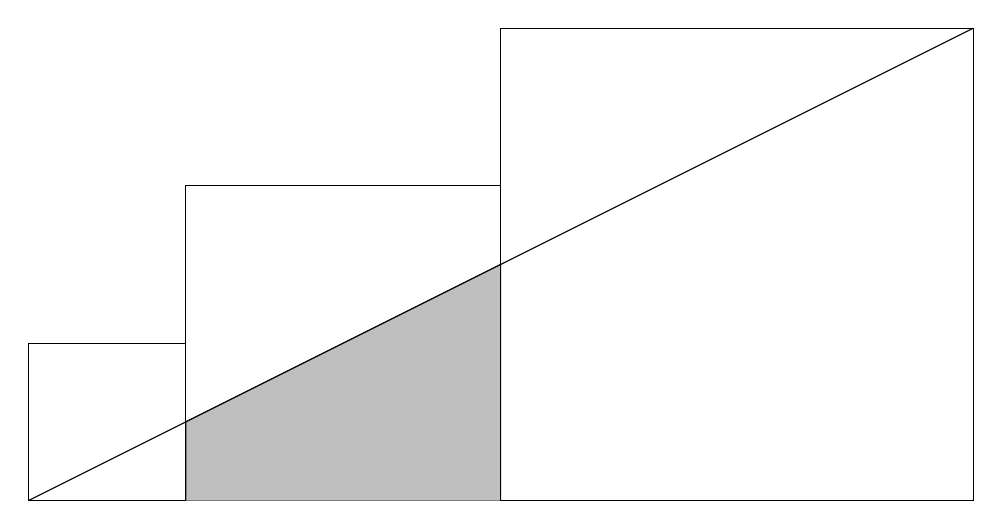
\begin{tikzpicture}
            \draw (0,0) -- (0,2) -- (2,2) -- (2,0) -- (2, 4) -- (6,4) -- (6,0) -- (6,6) -- (12,6) -- (12,0) -- (0,0);
            \draw (0,0) -- (12,6);
            \draw[fill=gray!50] (2,0) -- (2,1) -- (6, 3) -- (6,0);
        \end{tikzpicture}
        }
    \end{center}
\end{frame}


\refstepcounter{problem}
\begin{frame}[t, fragile]{Problem \thesection.\theproblem}
    \begin{block}{}[Mathcounts 2010 State, Sprint]
    The points (1, 7), (13, 16) and (5, $k$), where $k$ is an integer, are vertices of a triangle. What is the sum of the values of $k$ for which the area of the triangle is a minimum?
	
    \end{block}
\end{frame}

\refstepcounter{problem}
\begin{frame}[t, fragile]{Problem \thesection.\theproblem}
    \begin{block}{}[AMC 8, 2016]
    A semicircle is inscribed in an isosceles triangle with base $16$ and height $15$ so that the diameter of the semicircle is contained in the base of the triangle as shown. What is the radius of the semicircle? Express your answer as a common fraction.

	
    \end{block}
    \begin{center}
        \includegraphics[height=50mm,scale=0.25]{images/2016AMC8.png}
    \end{center}
\end{frame}

\refstepcounter{problem}
\begin{frame}[t, fragile]{Problem \thesection.\theproblem}
    \begin{block}{}[AJHSME, 1989]
    Suppose a square piece of paper is folded in half vertically.  The folded paper is then cut in half along the dashed line.  Three rectangles are formed-a large one and two small ones.  What is the ratio of the perimeter of one of the small rectangles to the perimeter of the large rectangle?

	
    \end{block}
    \begin{center}
        \includegraphics[height=50mm,scale=0.01]{images/1989_AJHSME_24.png}
    \end{center}
\end{frame}

\refstepcounter{problem}
\begin{frame}[t, fragile]{Problem \thesection.\theproblem}
    \begin{block}{}[Mathcounts 2008 State, Team]
    Circle $T$ has a circumference of $12\pi$ inches, and segment $XY$ is a diameter. If the measure of angle $TXZ$ is $60^\circ$, what is the length, in inches, of segment $XZ$?

	
    \end{block}
    \begin{center}
        \includegraphics[height=50mm,scale=0.25]{images/MC2008State_T5.png}
    \end{center}
\end{frame}


\refstepcounter{problem}
\begin{frame}[t, fragile]{Problem \thesection.\theproblem}
    \begin{block}{}[Mathcounts 2015 National, Sprint \#27]
     An equilateral triangle shares a side with a square, and a circle is inscribed between them, as shown. If the radius of the circle is $9 - 3\sqrt{3}$ , what is the side length of the square?
     

    \end{block}
    \begin{center}
        \begin{asy}
             unitsize (1cm);
             real r = 1, s = 3 + sqrt(3);
             pair O, A, B, C, D, E;
             O = (0, 0);
             A = (r, r);
             B = (r, r-s);
             C = (r-s, r-s);
             D = (r-s, r);
             E = rotate (-60, B)*C;
             
             draw(A--B--C--D--cycle);
             draw (B--E--C);
             draw(circle(O, r));
        \end{asy}
    \end{center}

\end{frame}

\refstepcounter{problem}
\begin{frame}[t, fragile]{Problem \thesection.\theproblem}
    \begin{block}{}[Mathcounts 2015 National, Sprint \#25]
     Right triangle $ABC$ has side lengths $AB = 4$ cm, $BC = 3$ cm
and $AC = 5$ cm. $A$ also is a vertex of a square, and $B$ and $C$ lie
on two sides of the square as shown. What is the area of the
square? Express your answer as a common fraction.

    \end{block}
    \begin{center}
        \begin{asy}
            import olympiad;
             unitsize (3cm);
             pair A, B, C, D, E, F;
           
             A = (1, 0);
             B = (0, 1/4);
             C = (3/16, 1);
             D = (1, 1);
             E = (0, 1);
             F = (0, 0);
             
             draw (A--B--C--cycle);
             draw (A--D--E--F--cycle);
             draw(rightanglemark(A, B, C, 2), black);
           
             label("$A$", A, SE);
             label("$B$", B, W);
             label ("$C$", C, N);
             
        \end{asy}
    \end{center}
    

\end{frame}

\refstepcounter{problem}
\begin{frame}[t, fragile]{Problem \thesection.\theproblem}
    \begin{block}{}[Mathcounts 2012 State, Sprint \#11]
    Triangle $MNO$ is an isosceles triangle with $MN=NO=25$ cm. A line segment, drawn from the midpoint of $\overline{MO}$ perpendicular to $\overline{MN}$, intersects $\overline{MN}$ at point $P$ with $NP:PM=4:1$. What is the length of the altitude drawn from point N to $\overline{MO}$? Express your answer in simplest radical form.
    \end{block}
    \begin{center}
        \includegraphics[height=50mm,scale=0.25]{11.png}
    \end{center}
    

\end{frame}

\refstepcounter{problem}
\begin{frame}[t, fragile]{Problem \thesection.\theproblem}
    \begin{block}{}
    (Mathcounts) A right square pyramid with base edges of length $8\sqrt{2}$ units each and slant edges of length 10 units each is cut by a plane that is parallel to its base and 3 units above its base. What is the volume, in cubic units, of the new pyramid that is cut off by this plane?
    \end{block}
    \begin{center}
        \includegraphics[scale=0.4]{56c724eb5297fe3abad02162d5be307b3f7e10f0.png}
    \end{center} 
    
\end{frame}

\refstepcounter{problem}
\begin{frame}[t, fragile]{Problem \thesection.\theproblem}
    \begin{block}{}
    (Purple Comet) Three lines are drawn parallel to each of the sides of triangle $ABC$
so that they intersect in the interior of $ \triangle ABC $. The resulting three smaller triangles have areas 1, 4, and 9. Find the area of triangle $ABC$. 

    \end{block}
    \begin{center}
        \begin{asy}
        import cse5;
        unitsize(0.75cm);
        
        pair A, B, C, D, E, F, G, H, I, J;
        real r1 = 1/2, r2 = 2/3;
        
        A = (0,0);
        B = (5,0);
        C = (3,7);
    
        E = (1/6)*(A + B);
        F = (4/6)*(A + B);
        
        G = (1/2)*(A + C);
        H = A + (2/3)*(C - A);
        
        I = (1/2)*(B + C);
        J = B + (5/6)*(C - B);
        
        D = G + (1/3)*(I - G);
        draw(A--B--C--A^^E--J^^F--H^^G--I);
        
        label("$A$", A, S);
        label("$B$", B, S);
        label("$C$", C, N);
        
        label("1", (D + G + H) / 3);
        label("4", (D + I + J) / 3);
        label("9", (D + E + F) / 3);
        
        
        \end{asy}
    \end{center}
        
    
\end{frame}

%-------------------------
\section{Challenge Practice Problems}

\refstepcounter{problem}
\begin{frame}[t, fragile]{Problem \thesection.\theproblem}
    \begin{block}{}[Mathcounts 2010 National, Target]
    A circle is inscribed in a rhombus, the lengths of whose diagonals are 2 feet and 4 feet. What is the area, in square feet, of the region of the rhombus that is outside the circular region? Express your answer as a decimal to the nearest tenth.
    \end{block}
    \begin{center}
        \includegraphics[height=50mm,scale=0.25]{images/2010MC_Nat_T5.png}
    \end{center}
	

\end{frame}

\refstepcounter{problem}
\begin{frame}[t, fragile]{Problem \thesection.\theproblem}
    \begin{block}{}[AIME I, 1994]
    A circle with diameter $\overline{PQ}$ of length 10 is internally tangent at $P$ to a circle of radius 20. Square $ABCD$ is constructed with $A$ and $B$ on the larger circle, $\overline{CD}$ tangent at $Q$ to the smaller circle, and the smaller circle outside $ABCD$. The length of $\overline{AB}$ can be written in the form $m + \sqrt{n}$, where $m$ and $n$ are integers. Find $m + n$.
    \end{block}
    \begin{center}
        \includegraphics[height=50mm,scale=0.25]{images/1994_AIME_2.png}
    \end{center}
	

\end{frame}

\refstepcounter{problem}
\begin{frame}[t, fragile]{Problem \thesection.\theproblem}
    \begin{block}{}[AIME II, 2009]
    Equilateral triangle $T$ is inscribed in circle $A$, which has radius $10$. Circle $B$ with radius $3$ is internally tangent to circle $A$ at one vertex of $T$. Circles $C$ and $D$, both with radius $2$, are internally tangent to circle $A$ at the other two vertices of $T$. Circles $B$, $C$, and $D$ are all externally tangent to circle $E$, which has radius $\dfrac mn$, where $m$ and $n$ are relatively prime positive integers. Find $m+n$.
    \end{block}
    \begin{center}
        \includegraphics[height=50mm,scale=0.25]{images/2009_AIME2_5.png}
    \end{center}
	

\end{frame}

\refstepcounter{problem}
\begin{frame}[t, fragile]{Problem \thesection.\theproblem}
    \begin{block}{}[Mathcounts]
    A circle is tangent to the positive $ x- $axis at $ x = 3 $. It passes through the distinct points $ (6, 6) $ and $ (p, p) $ where $ p $ is not 6. What is the value of $ p $? Express your answer as a common fraction.
	
    \end{block}
\end{frame}

\refstepcounter{problem}
\begin{frame}[t, fragile]{Problem \thesection.\theproblem}
    \begin{block}{}[Mathcounts National 2017, Sprint \#13]
     In right triangle $ABC$ with right angle at vertex $C$, a semicircle is constructed, as shown, with center $P$ on leg $AC$, so that the semicircle is tangent to leg $BC$ at $C$, tangent to the hypotenuse $AB$, and intersects leg $AC$ at $Q$ between $A$ and $C.$ The ratio of $AQ$ to $QC$ is $2:3.$ If $BC = 12,$ then what is the value of $AC?$ Express your answer in simplest radical form.    
    \end{block}
    \begin{center}
        \begin{asy}
            import olympiad;
            unitsize(0.25cm);
            pair A, B, C, O, T;
            real r = 24/sqrt(10);
            C = (0, 0);
            B = (0, 12);
            A = (-8*sqrt(10), 0);
            O = (-r, 0);
            T = foot(O, A, B);
            
            draw(A--B--C--cycle);
            draw(arc(O, r, 0, 180));
    
            dot(O);
            //dot(T);
            label("$A$", A, SW);
            label("$C$", C, SE);
            label("$B$", B, NE);
            label("$P$", O, S);
            label("$Q$", O*2, S);
            
        \end{asy}    
        \end{center}
        
    
\end{frame}

\refstepcounter{problem}
\begin{frame}[t, fragile]{Problem \thesection.\theproblem}
    \begin{block}{}[Mathcounts 2014 National Target \#8]
     A circle passes through two diagonally opposite vertices of a 3-inch by 4-inch rectangle. What is the least possible distance between the center of the circle and a vertex of the rectangle? Express your answer as a common fraction. 
	
    \end{block}
\end{frame}


\end{document}